\chapter{Implementation of the transformation}
\label{chap:implementation}
%===============================%
%         Trafo stages          %
%===============================%
In this chapter, some details of the transformation implementation will be presented. As mentioned before in section \ref{sec:vsdt}, the transformation process in the VSDT is divided into 5 stages. We've also mentioned that the default validation and structure mapping provided by the transformation framework are reuseable. For the implementation of the new transformation, the framework's DefaultBpmnValidator and BPMN2StrucBPMNTransformation are being reused, as we can see in Figure \ref{fig:implementation_stages}.

\begin{figure}[h]
	\centering		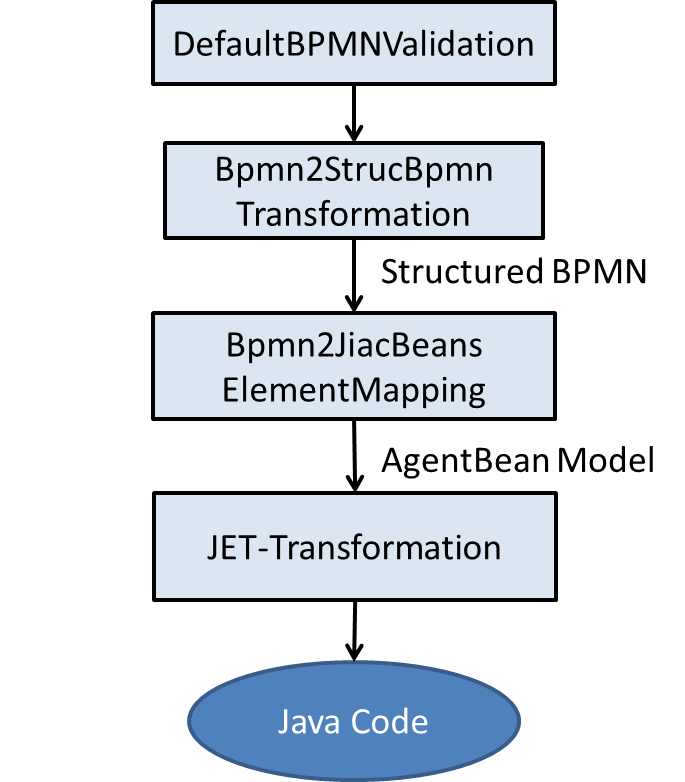
\includegraphics[width=0.5\textwidth]{images/implementation_stages.png}
	\caption{Transformation stages}
	\label{fig:implementation_stages}
\end{figure}

%===============================%
%           Metamodel           %
%===============================%
\section{AgentBean-Metamodel}
\begin{figure}[h]
	\centering		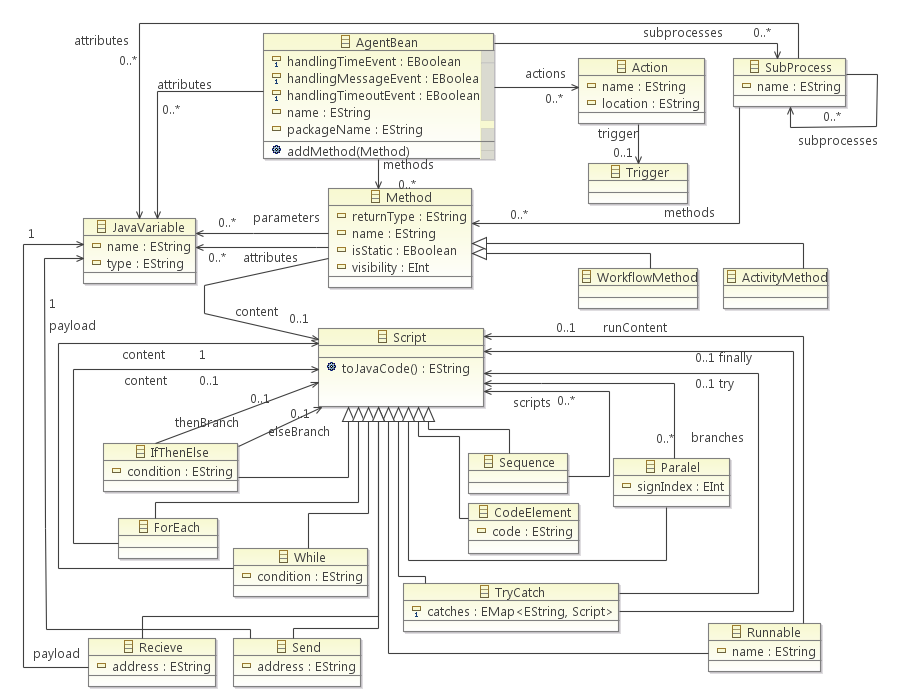
\includegraphics[width=1.0\textwidth]{images/agentBean_metamodel.png}
	\caption{AgentBean - Metamodel}
	\label{fig:agentbean_metamodel}
\end{figure}
